\subsection{Fully Connected layer} \label{subs:fcl}
The perceptron of section \ref{subs:perceptron} can be considered as a linear classifier for which the decision boundary is the hyperplane
$$ b + w_1 \cdot x_1 + ... + w_n \cdot x_n = 0$$
It is limited because it has only a linear boundary. For example, we can implement the boolean functions AND and OR, but it is impossible with the XOR function. To have a non-linear model, we must use a topology of perceptrons. The topology is composed of layers of perceptrons, each layer is called a \textbf{fully-connected layer} in the case of a \acrshort{cnn}. We can see an example on figure \ref{fig:fcn}.
\begin{figure}
    \centering
    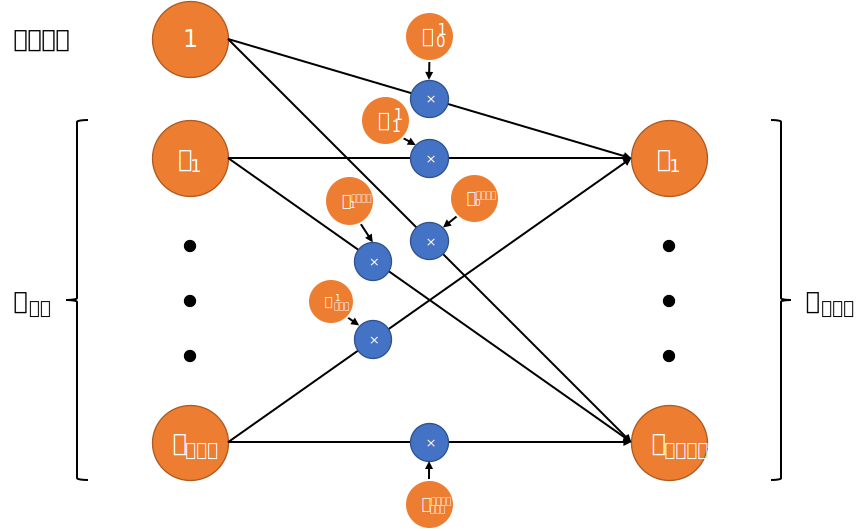
\includegraphics[width=\textwidth]{fcl.pdf}
    \caption{A fully connected layer}
    \label{fig:fcn}
\end{figure}

In the fully-connected layer, each neurons is connected to all the inputs or neurons of previous layers. A fully-connected layer is characterized by the number of neurons, activation functions, and the values of weights. We can express the outputs of such layer as
$$
\boldsymbol{y} = h(\boldsymbol{\bar{w}}^T \boldsymbol{\bar{x}}) \Leftrightarrow \forall o \in \{ 1, ..., N_{out} \} : y_o = h(\sum^{N_{in}}_{i=0} w^o_i \cdot x_i)
$$
where $\boldsymbol{\bar{x}}$ is the vector of the input of the layer, which can be output from another layer and $x_0 = 1$ because it is the biaises;   $\boldsymbol{\bar{w}}$ is the vector of all the weights of the layer, where $w^i_*$ are the weights of the ith perceptron and $w^*_0$ are the biases; and $\boldsymbol{h}$ is the activation function of the layer.

Usually, the fully-connected layers are placed at the end of the \acrshort{cnn}. It is used to classify the features of the convolutional layers which are converted as a one-dimension output \acrshort{fm}.
